\documentclass[12pt]{ximera}
\title{Cumulative Final (Version A)}
\begin{document}
\begin{abstract}
An archived 50-question cumulative final: voting methods, weighted voting and power indices, sealed bids, divider-chooser, Hamilton, Webster, and Huntington-Hill apportionment, and a mixed-strategy advertising game.
\end{abstract}
\maketitle

\section*{Cumulative Final (Version A)}

All $50$ questions are multiple choice. Round to two decimal places unless stated otherwise.

\begin{problem}
Questions 1--6 use the following preference schedule.
\begin{center}
\begin{tabular}{c|ccc}
Number of voters & 11 & 9 & 5\\\hline
1st & C & A & B\\
2nd & D & C & D\\
3rd & A & B & A\\
4th & B & D & C
\end{tabular}
\end{center}

\begin{prompt}
\textbf{1.} The winner under the Plurality method is:
\begin{multipleChoice}
\choice{Candidate A}
\choice{Candidate B}
\choice[correct]{Candidate C}
\choice{Candidate D}
\end{multipleChoice}
\begin{feedback}
First-place votes: C $11$, A $9$, B $5$, D $0$.
\end{feedback}
\end{prompt}

\begin{prompt}
\textbf{2.} The winner under Plurality-with-Elimination is:
\begin{multipleChoice}
\choice[correct]{Candidate A}
\choice{Candidate B}
\choice{Candidate C}
\choice{Candidate D}
\end{multipleChoice}
\begin{feedback}
No majority ($13$). D ($0$) and then B ($5$) are eliminated; B's voters go to A (D is gone), giving A $14$, C $11$.
\end{feedback}
\end{prompt}

\begin{prompt}
\textbf{3.} Using the Borda count, the winner is:
\begin{multipleChoice}
\choice{Candidate A}
\choice{Candidate B}
\choice[correct]{Candidate C}
\choice{Candidate D}
\end{multipleChoice}
\end{prompt}

\begin{prompt}
\textbf{4.} Using the Borda count, the second place is:
\begin{multipleChoice}
\choice[correct]{Candidate A}
\choice{Candidate B}
\choice{Candidate C}
\choice{Candidate D}
\end{multipleChoice}
\end{prompt}

\begin{prompt}
\textbf{5.} Using the Borda count, the third place is:
\begin{multipleChoice}
\choice{Candidate A}
\choice{Candidate B}
\choice{Candidate C}
\choice[correct]{Candidate D}
\end{multipleChoice}
\end{prompt}

\begin{prompt}
\textbf{6.} Using the Borda count, the fourth place is:
\begin{multipleChoice}
\choice{Candidate A}
\choice[correct]{Candidate B}
\choice{Candidate C}
\choice{Candidate D}
\end{multipleChoice}
\begin{feedback}
Borda points: C $76$, A $68$, D $57$, B $49$.
\end{feedback}
\end{prompt}
\end{problem}

\begin{problem}
Questions 7--11 use the Pairwise Comparisons method on this preference schedule.
\begin{center}
\begin{tabular}{c|cccc}
Number of voters & 5 & 4 & 2 & 1\\\hline
1st & B & D & A & C\\
2nd & C & B & D & B\\
3rd & D & A & C & A\\
4th & A & C & B & D
\end{tabular}
\end{center}

\begin{prompt}
\textbf{7.} The winner is:
\begin{multipleChoice}
\choice{Candidate A}
\choice[correct]{Candidate B}
\choice{Candidate C}
\choice{Candidate D}
\end{multipleChoice}
\end{prompt}

\begin{prompt}
\textbf{8.} The second place is:
\begin{multipleChoice}
\choice{Candidate A}
\choice{Candidate B}
\choice{Candidate C}
\choice[correct]{Candidate D}
\end{multipleChoice}
\end{prompt}

\begin{prompt}
\textbf{9.} The third place is:
\begin{multipleChoice}
\choice{Candidate A}
\choice{Candidate B}
\choice[correct]{Candidate C}
\choice{Candidate D}
\end{multipleChoice}
\end{prompt}

\begin{prompt}
\textbf{10.} The fourth place is:
\begin{multipleChoice}
\choice[correct]{Candidate A}
\choice{Candidate B}
\choice{Candidate C}
\choice{Candidate D}
\end{multipleChoice}
\begin{feedback}
B beats A $10$--$2$ and C $9$--$3$ and ties D $6$--$6$: $2.5$. D beats A $9$--$3$, ties B and C: $2$. C ties A and D: $1$. A ties C: $0.5$.
\end{feedback}
\end{prompt}

\begin{prompt}
\textbf{11.} A Condorcet candidate for this election
\begin{multipleChoice}
\choice{is A}
\choice{is B}
\choice{is C}
\choice{is D}
\choice[correct]{does not exist}
\end{multipleChoice}
\begin{feedback}
No: B, the Pairwise winner, only ties D.
\end{feedback}
\end{prompt}
\end{problem}

\begin{problem}
An election with four candidates and $40$ voters used a modified Borda count: $7,5,3,1$ points. B had $250$ points, C $90$, and D $110$. Questions 12--15 ask for the ranking.

\begin{prompt}
\textbf{12.} The winner is:
\begin{multipleChoice}
\choice{Candidate A}
\choice[correct]{Candidate B}
\choice{Candidate C}
\choice{Candidate D}
\end{multipleChoice}
\end{prompt}

\begin{prompt}
\textbf{13.} The second place is:
\begin{multipleChoice}
\choice[correct]{Candidate A}
\choice{Candidate B}
\choice{Candidate C}
\choice{Candidate D}
\end{multipleChoice}
\end{prompt}

\begin{prompt}
\textbf{14.} The third place is:
\begin{multipleChoice}
\choice{Candidate A}
\choice{Candidate B}
\choice{Candidate C}
\choice[correct]{Candidate D}
\end{multipleChoice}
\end{prompt}

\begin{prompt}
\textbf{15.} The fourth place is:
\begin{multipleChoice}
\choice{Candidate A}
\choice{Candidate B}
\choice[correct]{Candidate C}
\choice{Candidate D}
\end{multipleChoice}
\begin{feedback}
Each ballot awards $16$ points, $640$ in all, so A has $640-450=190$: B $250$, A $190$, D $110$, C $90$.
\end{feedback}
\end{prompt}
\end{problem}

\begin{problem}
Questions 16--19 use the weighted voting system $[20:10,7,5,3,1]$.

\begin{prompt}
\textbf{16.} Does this system have a dictator?
\begin{multipleChoice}
\choice{Yes}
\choice[correct]{No}
\choice{Can't be determined}
\end{multipleChoice}
\begin{feedback}
No player's weight reaches the quota of $20$.
\end{feedback}
\end{prompt}

\begin{prompt}
\textbf{17.} Which players have veto power?
\begin{multipleChoice}
\choice{All players}
\choice{Only $P_1$}
\choice{Only $P_2$}
\choice[correct]{$P_1$ and $P_2$}
\choice{None of the players}
\end{multipleChoice}
\begin{feedback}
Without $P_1$: $16<20$; without $P_2$: $19<20$; without $P_3$: $21\ge20$.
\end{feedback}
\end{prompt}

\begin{prompt}
\textbf{18.} How many coalitions of two or more players are there?
\begin{multipleChoice}
\choice{$5$}
\choice{$32$}
\choice{$31$}
\choice[correct]{$26$}
\end{multipleChoice}
\begin{feedback}
$2^5-5-1=26$.
\end{feedback}
\end{prompt}

\begin{prompt}
\textbf{19.} How many sequential coalitions are there?
\begin{multipleChoice}
\choice{$121$}
\choice[correct]{$120$}
\choice{$119$}
\choice{$24$}
\end{multipleChoice}
\begin{feedback}
$5!=120$.
\end{feedback}
\end{prompt}
\end{problem}

\begin{problem}
Questions 20--23 use the weighted voting system $[8:6,3,2]$.

\begin{prompt}
\textbf{20.} Which are the winning coalitions?
\begin{multipleChoice}
\choice{$\set{P_1,P_2}$ and $\set{P_1,P_3}$ only}
\choice[correct]{$\set{P_1,P_2}$, $\set{P_1,P_3}$, and $\set{P_1,P_2,P_3}$ only}
\choice{$\set{P_1,P_2,P_3}$ only}
\choice{$\set{P_1,P_2}$, $\set{P_1,P_3}$, and $\set{P_2,P_3}$ only}
\end{multipleChoice}
\begin{feedback}
$\set{P_1,P_2}=9$, $\set{P_1,P_3}=8$, $\set{P_1,P_2,P_3}=11$; but $\set{P_2,P_3}=5$ loses.
\end{feedback}
\end{prompt}

\begin{prompt}
\textbf{21.} Which player(s) have the highest critical count?
\begin{multipleChoice}
\choice[correct]{$P_1$}
\choice{$P_2$}
\choice{$P_3$}
\choice{All are equal}
\choice{$P_1$ and $P_2$}
\end{multipleChoice}
\begin{feedback}
$P_1$ is critical in all three winning coalitions; $P_2$ only in $\set{P_1,P_2}$ and $P_3$ only in $\set{P_1,P_3}$.
\end{feedback}
\end{prompt}

\begin{prompt}
\textbf{22.} Are there any dummy players?
\begin{multipleChoice}
\choice{Yes}
\choice[correct]{No}
\choice{No way to tell}
\end{multipleChoice}
\begin{feedback}
No: every player is critical at least once.
\end{feedback}
\end{prompt}

\begin{prompt}
\textbf{23.} What is the Banzhaf power distribution?
\begin{multipleChoice}
\choice{$\beta_1=\beta_2=\beta_3=\frac13$}
\choice{$\beta_1=\beta_2=\beta_3=\frac15$}
\choice[correct]{$\beta_1=\frac35$, $\beta_2=\frac15$, $\beta_3=\frac15$}
\choice{$\beta_1=\frac35$, $\beta_2=\frac25$, $\beta_3=0$}
\end{multipleChoice}
\begin{feedback}
Critical counts $3,1,1$ out of $5$.
\end{feedback}
\end{prompt}
\end{problem}

\begin{problem}
In a weighted voting system with four players, the only winning coalitions are
\[
\set{P_1,P_2},\ \set{P_1,P_2,P_3},\ \set{P_1,P_2,P_4},\ \set{P_1,P_3,P_4},\ \set{P_1,P_2,P_3,P_4}.
\]

\begin{prompt}
\textbf{24.} Which player(s) have the highest critical count?
\begin{multipleChoice}
\choice[correct]{$P_1$}
\choice{$P_2$}
\choice{$P_3$}
\choice{$P_4$}
\choice{None of these}
\end{multipleChoice}
\begin{feedback}
Critical players: both in $\set{P_1,P_2}$; $P_1,P_2$ in $\set{P_1,P_2,P_3}$ and in
$\set{P_1,P_2,P_4}$; all three in $\set{P_1,P_3,P_4}$; only $P_1$ in the grand coalition
(since $\set{P_2,P_3,P_4}$ loses). Counts $5,3,1,1$.
\end{feedback}
\end{prompt}

\begin{prompt}
\textbf{25.} Are there any dummy players?
\begin{multipleChoice}
\choice{Yes}
\choice[correct]{No}
\choice{No way to tell}
\end{multipleChoice}
\end{prompt}

\begin{prompt}
\textbf{26.} What is the Banzhaf power distribution?
\begin{multipleChoice}
\choice{all $\frac14$}
\choice{all $\frac6{24}$}
\choice{$\frac4{10},\frac4{10},\frac1{10},\frac1{10}$}
\choice[correct]{$\frac5{10},\frac3{10},\frac1{10},\frac1{10}$}
\choice{$\frac5{10},\frac3{10},\frac2{10},0$}
\end{multipleChoice}
\end{prompt}
\end{problem}

\begin{problem}
List the sequential coalitions of the weighted voting system $[9:7,5,1]$ and find the Shapley-Shubik power distribution.

\begin{prompt}
\textbf{27.} Which player(s) have the highest pivotal count?
\begin{multipleChoice}
\choice{$P_1$}
\choice{$P_2$}
\choice{$P_2$ and $P_3$}
\choice[correct]{$P_1$ and $P_2$}
\choice{All are equal}
\end{multipleChoice}
\begin{feedback}
Pivots: $\seq{P_1,\underline{P_2},P_3}$, $\seq{P_1,P_3,\underline{P_2}}$,
$\seq{P_2,\underline{P_1},P_3}$, $\seq{P_2,P_3,\underline{P_1}}$, $\seq{P_3,P_1,\underline{P_2}}$,
$\seq{P_3,P_2,\underline{P_1}}$. $P_1$ and $P_2$ are pivotal $3$ times each, $P_3$ never.
\end{feedback}
\end{prompt}

\begin{prompt}
\textbf{28.} Are there any dummy players?
\begin{multipleChoice}
\choice[correct]{Yes}
\choice{No}
\choice{No way to tell}
\end{multipleChoice}
\begin{feedback}
Yes: $P_3$ is never pivotal.
\end{feedback}
\end{prompt}

\begin{prompt}
\textbf{29.} What is the Shapley-Shubik power distribution?
\begin{multipleChoice}
\choice{$\sigma_1=\sigma_2=\frac26$, $\sigma_3=0$}
\choice{all $\frac26$}
\choice{$\frac36,\frac26,\frac16$}
\choice{$\frac46,\frac16,\frac16$}
\choice[correct]{$\frac36,\frac36,0$}
\end{multipleChoice}
\end{prompt}
\end{problem}

\begin{problem}
Andre, Bea, and Chad divide an estate consisting of a house and a small farm by sealed
bids.
\begin{center}
\begin{tabular}{l|rrr}
 & Andre & Bea & Chad\\\hline
House & \$151,000 & \$145,000 & \$175,000\\
Farm & \$431,000 & \$425,000 & \$428,000
\end{tabular}
\end{center}

\begin{prompt}
\textbf{30.} After the first settlement, what is each player's share of the surplus?
\begin{multipleChoice}
\choice{\$21,000}
\choice{There was no surplus}
\choice{\$8,000}
\choice[correct]{\$7,000}
\end{multipleChoice}
\begin{feedback}
Totals $582$, $570$, $603$ (thousands), so fair shares are $194$, $190$, $201$. Andre gets the farm ($431$) and owes $237$; Bea receives $190$; Chad gets the house ($175$) and receives $26$. Surplus $237-190-26=21$, or $7$ each.
\end{feedback}
\end{prompt}

\begin{prompt}
\textbf{31.} What does Andre get?
\begin{multipleChoice}
\choice{The farm and some cash}
\choice{Only \$194,000 cash}
\choice{The farm only}
\choice{The house and \$237,000}
\choice[correct]{The farm, and pays \$230,000}
\end{multipleChoice}
\end{prompt}

\begin{prompt}
\textbf{32.} What does Bea get?
\begin{multipleChoice}
\choice{The farm, and pays \$215,000}
\choice{Only \$190,000 cash}
\choice{The house and some cash}
\choice[correct]{Only \$197,000 cash}
\choice{The house, and pays \$197,000}
\end{multipleChoice}
\end{prompt}

\begin{prompt}
\textbf{33.} What does Chad get?
\begin{multipleChoice}
\choice{The house, and pays \$33,000}
\choice{Only \$201,000 cash}
\choice{The farm only}
\choice{The house and \$26,000}
\choice[correct]{The house and \$33,000}
\end{multipleChoice}
\begin{feedback}
Final: Andre pays $237-7=230$; Bea receives $190+7=197$; Chad receives $26+7=33$.
\end{feedback}
\end{prompt}
\end{problem}

\begin{problem}
Jared and Karla bought a foot-long sub, vegetarian on $[0,6]$ and meatball on $[6,12]$:
\begin{center}
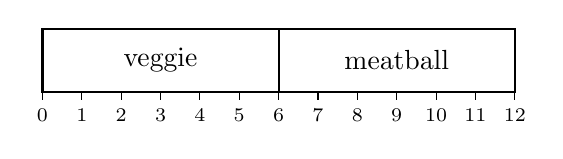
\begin{tikzpicture}
\draw[thick] (0,0) rectangle (6,0.8); \draw[thick] (3,0) -- (3,0.8);
\node at (1.5,0.4) {veggie}; \node at (4.5,0.4) {meatball};
\foreach \x in {0,...,12} \draw (\x/2,0) -- (\x/2,-0.1) node[below,font=\scriptsize] {\x};
\end{tikzpicture}
\end{center}
Jared likes meatball three times as much as veggie. They use the divider-chooser method
with a single cut across the sub.

\begin{prompt}
\textbf{34.} If Jared divides, which piece is worth exactly $50\%$ to him?
\begin{multipleChoice}
\choice{$[0,6]$}
\choice{$[4,12]$}
\choice[correct]{$[0,8]$}
\choice{$[6,12]$}
\choice{None of these}
\end{multipleChoice}
\begin{feedback}
To Jared veggie is worth $\frac14$ and meatball $\frac34$, or $\frac18$ per inch of meatball. $[0,8]$: $\frac14+2\cdot\frac18=\frac12$.
\end{feedback}
\end{prompt}

\begin{prompt}
\textbf{35.} If Karla divides and is a strict vegetarian, which piece is worth exactly $50\%$ to her?
\begin{multipleChoice}
\choice{$[0,6]$}
\choice{$[6,12]$}
\choice[correct]{$[3,12]$}
\choice{$[8,12]$}
\choice{None of these}
\end{multipleChoice}
\begin{feedback}
$[3,12]$ holds half of the veggie, which is all she values.
\end{feedback}
\end{prompt}

\begin{prompt}
\textbf{36.} Suppose instead Karla likes veggie three times as much as meatball. How should she cut?
\begin{multipleChoice}
\choice{$s_1=[0,6]$, $s_2=[6,12]$}
\choice{$s_1=[0,3]$, $s_2=[3,12]$}
\choice[correct]{$s_1=[0,4]$, $s_2=[4,12]$}
\choice{$s_1=[0,8]$, $s_2=[8,12]$}
\choice{$s_1=[0,7.5]$, $s_2=[7.5,12]$}
\end{multipleChoice}
\begin{feedback}
Veggie is worth $\frac34$ to her, $\frac18$ per inch, so $[0,4]$ is worth $\frac12$.
\end{feedback}
\end{prompt}

\begin{prompt}
\textbf{37.} After Karla's cut in question 36, Jared picks his better share. What is it worth to him?
\begin{multipleChoice}
\choice[correct]{$\frac56$}
\choice{$\frac13$}
\choice{$\frac12$}
\choice{$\frac{11}{12}$}
\choice{$\frac14$}
\end{multipleChoice}
\begin{feedback}
$[4,12]$: $\frac2{6}\cdot\frac14+\frac34=\frac1{12}+\frac9{12}=\frac56$.
\end{feedback}
\end{prompt}
\end{problem}

\begin{problem}
The Kingdom of Arendelle has five states. Their populations, as percentages of the
total, are below. Use Hamilton's method to apportion $400$ seats.
\begin{center}
\begin{tabular}{l|cccccc}
State & A & B & C & D & E & Total\\\hline
Population (\%) & 10.11 & 13 & 41.22 & 20 & 15.67 & 100
\end{tabular}
\end{center}

\begin{prompt}
\textbf{38.} The standard divisor, as a percent of the population, is:
\begin{multipleChoice}
\choice{$80$}
\choice{$25$}
\choice[correct]{$0.25$}
\choice{$4$}
\end{multipleChoice}
\begin{feedback}
$100/400=0.25$.
\end{feedback}
\end{prompt}

\begin{prompt}
\textbf{39.} After the first step, how many surplus seats are there?
\begin{multipleChoice}
\choice{None}
\choice{$1$}
\choice[correct]{$2$}
\choice{$3$}
\choice{Not enough seats to give out}
\end{multipleChoice}
\begin{feedback}
Quotas $40.44$, $52$, $164.88$, $80$, $62.68$; lower quotas total $398$.
\end{feedback}
\end{prompt}

\begin{prompt}
\textbf{40.} The final apportionment (A, B, C, D, E) is:
\begin{multipleChoice}
\choice{$40,52,164,80,62$}
\choice{$41,52,165,80,62$}
\choice{$41,52,165,80,63$}
\choice[correct]{$40,52,165,80,63$}
\end{multipleChoice}
\begin{feedback}
The two surplus seats go to the largest residues: C ($0.88$) and E ($0.68$).
\end{feedback}
\end{prompt}
\end{problem}

\begin{problem}
A small country with five states apportions $23$ seats in its congress.
\begin{center}
\begin{tabular}{l|cccccc}
State & A & B & C & D & E & Total\\\hline
Population & 13,475 & 52,085 & 30,085 & 11,792 & 19,063 & 126,500
\end{tabular}
\end{center}

\begin{prompt}
\textbf{41.} What is the standard divisor?
\begin{multipleChoice}
\choice{$5{,}000$}
\choice{$126{,}000$}
\choice{$23$}
\choice[correct]{$5{,}500$}
\choice{None of these}
\end{multipleChoice}
\begin{feedback}
Quotas: $2.45$, $9.47$, $5.47$, $2.144$, $3.466$.
\end{feedback}
\end{prompt}

\begin{prompt}
\textbf{42.} With Webster's method, how many seats are handed out in the first step?
\begin{multipleChoice}
\choice{Exactly $23$ (no surplus)}
\choice[correct]{Only $21$ ($2$ surplus)}
\choice{Too many: $25$}
\choice{None of these}
\end{multipleChoice}
\begin{feedback}
Conventional rounding gives $2,9,5,2,3=21$.
\end{feedback}
\end{prompt}

\begin{prompt}
\textbf{43.} To finish with Webster's method, we would:
\begin{multipleChoice}
\choice{be done after the first step}
\choice{seek a divisor bigger than the SD}
\choice[correct]{seek a divisor smaller than the SD}
\choice{give the surplus seats to the largest residues}
\choice{none of these}
\end{multipleChoice}
\begin{feedback}
Too few seats, so the quotas must grow, which needs a smaller divisor.
\end{feedback}
\end{prompt}

\begin{prompt}
\textbf{44.} With Huntington-Hill, how many seats are handed out in the first step?
\begin{multipleChoice}
\choice[correct]{Exactly $23$ (no surplus)}
\choice{Only $21$ ($2$ surplus)}
\choice{Too many: $25$}
\choice{None of these}
\end{multipleChoice}
\begin{feedback}
Cutoffs: $\sqrt{6}\approx2.4495$, $\sqrt{90}\approx9.4868$, $\sqrt{30}\approx5.4772$, $\sqrt6\approx2.4495$, $\sqrt{12}\approx3.4641$. A ($2.45$) and E ($3.466$) are just above their cutoffs, giving $3,9,5,2,4=23$.
\end{feedback}
\end{prompt}

\begin{prompt}
\textbf{45.} To finish with Huntington-Hill, we would:
\begin{multipleChoice}
\choice[correct]{be done after the first step}
\choice{seek a divisor bigger than the SD}
\choice{seek a divisor smaller than the SD}
\choice{give the surplus seats to the largest residues}
\choice{none of these}
\end{multipleChoice}
\end{prompt}
\end{problem}

\begin{problem}
Allied Manufacturing (A) and its competitor Bates Manufacturing (B) each launch a T.V.
or radio advertising campaign. The payoff matrix shows Allied's increased sales, in
millions (and Bates's matching losses):
\[
\begin{array}{r|rr}
 & \text{B: T.V.} & \text{B: Radio}\\\hline
\text{A: T.V.} & 3.0 & -2.1\\
\text{A: Radio} & -1.0 & 1.2
\end{array}
\]
Let $p_1$ be the probability that Allied chooses T.V.

\begin{prompt}
\textbf{46.} Allied's expected value if Bates picks T.V.:
\begin{multipleChoice}
\choice{$3p_1+1-p_1$}
\choice[correct]{$4p_1-1$}
\choice{$-0.9p_1-1.2$}
\choice{$-3.3p_1+1.2$}
\choice{None of these}
\end{multipleChoice}
\end{prompt}

\begin{prompt}
\textbf{47.} Allied's expected value if Bates picks radio:
\begin{multipleChoice}
\choice{$3p_1+1-p_1$}
\choice{$4p_1-1$}
\choice{$-0.9p_1-1.2$}
\choice[correct]{$-3.3p_1+1.2$}
\choice{None of these}
\end{multipleChoice}
\begin{feedback}
T.V.: $3p_1-1(1-p_1)=4p_1-1$. Radio: $-2.1p_1+1.2(1-p_1)=-3.3p_1+1.2$.
\end{feedback}
\end{prompt}

\begin{prompt}
\textbf{48.} The optimal value of $p_1$ is:
\begin{multipleChoice}
\choice[correct]{$0.30$}
\choice{$0.04$}
\choice{$-0.04$}
\choice{$0.75$}
\choice{$0.50$}
\end{multipleChoice}
\begin{feedback}
$4p_1-1=-3.3p_1+1.2$ gives $7.3p_1=2.2$, so $p_1\approx0.30$.
\end{feedback}
\end{prompt}

\begin{prompt}
\textbf{49.} Which strategy is Allied more likely to pick?
\begin{multipleChoice}
\choice{T.V.}
\choice[correct]{Radio}
\choice{Equally likely}
\end{multipleChoice}
\begin{feedback}
$p_1\approx0.30<0.5$, so radio $70\%$ of the time.
\end{feedback}
\end{prompt}

\begin{prompt}
\textbf{50.} Is this a strictly determined game?
\begin{multipleChoice}
\choice{Yes}
\choice[correct]{No}
\end{multipleChoice}
\begin{feedback}
No. The row minimums $-2.1,-1.0$ have maximum $-1.0$; the column maximums $3.0,1.2$ have minimum $1.2$. They differ, so there is no saddle point.
\end{feedback}
\end{prompt}
\end{problem}

\end{document}
